\documentclass{beamer}
\setbeamertemplate{navigation symbols}{}
\setbeamertemplate{bibliography item}[text]

\usepackage{beamerthemeshadow}
\usepackage{amsmath}
\usepackage{amssymb}
\usepackage{graphicx}
\graphicspath{ {./images/} }
\begin{document}
\title{Farkas Lemma}  
\author{Coman Florin-Alexandru}

\begin{frame}
\titlepage
\end{frame}

\begin{frame}\frametitle{Table of contents}\tableofcontents
\end{frame}

\section{Farkas Lemma}
\subsection{Farkas Lemma, Version I}
\begin{frame}\frametitle{Farkas Lemma, Version I}
\begin{block}{Lemma 1.1. (Farkas Lemma, Version I)}
Given any $d \times n$ real matrix, $A$, and any vector, $z \in \mathbb{R}^d$, exactly one of the following alternatives occurs: \\
$(a)$ The linear system, $A x = z$, has a solution, $x = (x_1, ... , x_n)$ such that $x \geq 0$ and $x_1 + ... + x_n = 1$, or \\
$(b)$ There is some $c \in \mathbb{R}^d$ and some $\alpha \in ]mathbb{R}$ such that $c^T z < \alpha$ and $c^T A \geq \alpha.$ 
\end{block}
\end{frame}

\begin{frame}\frametitle{Farkas Lemma, Version I}
\begin{block}{Remark}
If we relax the requirements on solution of $A x = z$ and only require $x \geq 0$ ($x_1 + ... + x_n = 1$ is no longer required) then, in condition $(b)$, we can take $\alpha = 0$. This is another verion of Farkas Lemma.
\end{block}
\begin{block}{}
In this case, instead of considering the convex hull of $\lbrace A_1, ... A_n \rbrace$ we are considering the convex cone, \\
\centerline{$cone(A_1, ... , A_n) = \lbrace \lambda A_1 + ... + \lambda_n A_n | \lambda_i \geq 0, 1 \leq i \leq n \rbrace$,}
that is, we are dropping the condition $\lambda_1 + ... + \lambda_n = 1$. 
\end{block}
\end{frame}

\begin{frame}\frametitle{Farkas Lemma, Version I}
\begin{block}{}
For this version of Farkas Lemma we need the following separation lemma:
\end{block}
\begin{block}{Proposition 1.1.}
Let $C \subseteq \mathbb{E}^d$ be any closed convex cone with vertex $O$. Then, for every point, $a$, not in $C$, there is a hyperplane, $H$, passing through $O$ separating $a$ and $C$ with $a \notin H.$
\end{block}
\begin{block}{}
\begin{figure}[h]
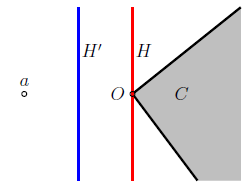
\includegraphics[width=3.5cm]{picture1}
\end{figure}
\fontsize{6.5pt}{7.2}\selectfont
\centerline{\textbf{Figure 1.} Illustration for Proposition 1.1.}
\end{block}
\end{frame}

\subsection{Farkas Lemma, Version II}
\begin{frame}\frametitle{Farkas Lemma, Version II}
\begin{block}{Lemma 1.2. (Farkas Lemma, Version II)}
Given any $d \times n$ real matrix, $A$, and any vector, $z \in \mathbb{R}^d$, exactly one of the following alternatives occurs: \\
$(a)$ The linear system, $A x = z$, has a solution, $x$, such that $x \geq 0$, or \\
$(b)$ There is some $c \in \mathbb{R}^d$ such that $c^T z < 0$ and $c^T A \geq 0.$
\end{block}
\end{frame}

\subsection{Farkas Lemma, Version III}
\begin{frame}\frametitle{Farkas Lemma, Version III}
\begin{block}{Lemma 1.3. (Farkas Lemma, Version III)}
Given any $d \times n$ real matrix, $A$, and any vector, $z \in \mathbb{R}^d$, exactly one of the following alternatives occurs: \\
$(a)$ The system of inequalities, $A x \leq z$, has a solution, $x$, or \\
$(b)$ There is some $c \in \mathbb{R}^d$ such that $c \geq 0$, $c^T z < 0$ and $c^T A = 0$.
\end{block}
\end{frame}

\begin{frame}\frametitle{Farkas Lemma, Version III}
\begin{block}{Proof I}
The proof uses two tricks from linear programming: \\
1. We convert the system of inequalities, $A x \leq z$, into a system of equations by introducing a vector of \textbf{slack variables}, $γ = (γ_1, . . . , γ_d)$, where the system of equations is \\
\centerline{$(A, I)\begin{pmatrix}
x \\
\gamma
\end{pmatrix} = z$,}
with $\gamma \geq 0$. \\
2. We replace each "uncontrained variable", $x_i$, by $x_i = X_i - Y_i$, with $X_i, Y_I \geq 0$.
\end{block}
\end{frame}

\begin{frame}\frametitle{Farkas Lemma, Version III}
\begin{block}{Proof II}
Then, the original system $A x \leq z$ has a solution, $x$ (unconstrained), iff the systen of equations \\
\centerline{$(A, -A, I)\begin{pmatrix}
X \\
Y \\
\gamma
\end{pmatrix} = z$}
has a solution with $X, Y, \gamma \geq 0$.
\end{block}
\begin{block}{}
By Farkas II, this system has no solution iff there exists some $c \in \mathbb{R}^d$ with $c^T z < 0$ and \\
\centerline{$c^T (A, -A, I) \geq 0$,}
that is, $c^T A \geq 0$. $- c^T A \geq 0$, and $c \geq 0$. \\
However, these four conditions reduce to $c^T z < 0$, $c^T A = 0$ and $c \geq 0$.
\end{block}
\end{frame}

\section{Bibliography}
\begin{frame}[allowframebreaks]
\frametitle{Bibliography}
    \tiny{\bibliographystyle{abbrv} }
    \bibliography{main}
\end{frame}

\end{document}